Project Iris will consist of four major layers. Tracking, Viewer, Calibration, and the Device. 

\begin{figure}[h!]
	\centering
 	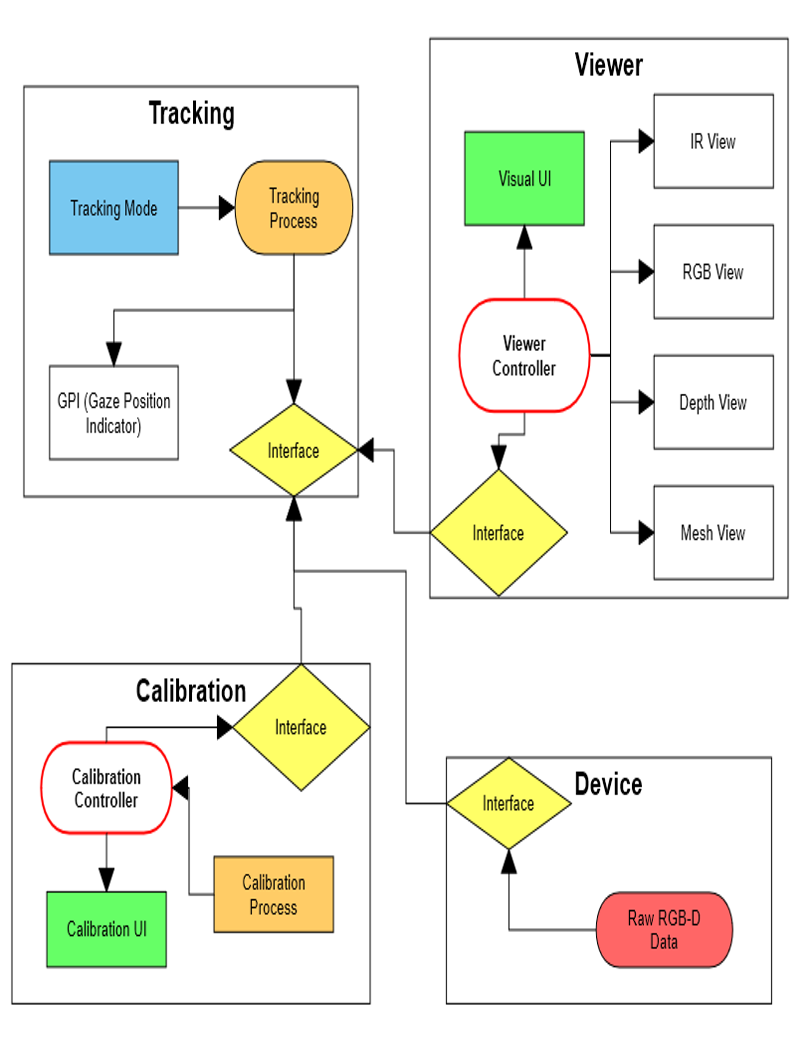
\includegraphics[width=0.60\textwidth]{images/system-architecture}
 \caption{Project Iris architectural layer diagram}
\end{figure}

\subsection{Tracking Description}
The tracking layer is the most important layer of the architecture. It is where the most important work will be done for Project Iris. This layer consist of the tracking process, which determines where on the screen the software believes the gaze is located. This layer uses calibration data from the calibration layer, data from the device layer, and receives commands from the interface (i.e. start/stop).

\subsection{Viewer Description}
The viewer layer provides a GUI for the user, and a way to control Project Iris. It receives camera data trough the tracking layer and can display it for the user.

\subsection{Calibration Description}
The calibration layer outputs data to the screen with a UI and uses data from the device layer to build a calibration profile of a user. This calibration data is the given to the tracking layer.

\subsection{Device Description}
The device layer consist of the drivers for the SR300. This layer is the simplest as its interactions with the other layers are purely to send its data to them. 